\section{hadoop}
yahoo的hadoop的设计:https://developer.yahoo.com/hadoop/tutorial/module1.html
hadoop的优势和劣势,hadoop正对的应用,yahoo的hadoop等


\subsection{背景}
对于超大数据的处理,input data很难之存放在一个单独的计算机上,而且内存也不够。因为hadoop有一个HDFS,分布式文件系统,将input data分成多个块,然后存放集群中的多个机器上。

执行超大数据的计算非常困难。必须处理好多个机器上的并发问题,比如需要相互合作,有可能其中一个机器出现问题。如果在单机上出现错误,程序员不会考虑这个问题,因为没有办法恢复。

但是在分布式环境下,parital failures是非常常见的情况,例如cluster中individual compute节点出现,overheat, crash, hard drive failures, run out of memory or disk space.例如数据有可能是破坏的,恶意的,甚至不适合提交的。多个client也许会有所不同,clock不同步。
分布式环境在遇到这些错误的时候,系统能够恢复,并且继续下一部的计算

不同的分布式系统提供不同的方式处理错误,
Hadoop provides no security model, nor safeguards against malicously inserted data.
Hadoop能够处理hardware failure and data congestion问题

处理以上问题,每个计算机的hardware资源是有限的,主要的资源包括:
\begin{itemize}
  \item Processor time
  \item Memory:对于超大数据,要求很大的memory,单机上无法满足
  \item Hard drive space
  \item NetWork bandwidth: bandwidth is a scarce resource even on an internal network.
\end{itemize}

分布式系统中的各节点间的同步(Synchronization)是设计分布式系统最大的挑战。

设计分布式系统如此多的挑战,为什么还一定要使用分布式系统呢?虽然多核机器可以做到足够的好,一个芯片上有很多个cores,但问题在于,输入数据的传输速度远比数据处理的速度慢,cores大部分时间在等待。

\subsection{hadoop的原理}
Hadoop is designed to efficiently process large volumes of information by connecting many commodity computers together to work in parallel.

Hadoop的最大特色就是它"simplified programming model",user可以快速的写,测试。Hadoop的efficient, automatic distribution of data and work across machines and in turn utilizing the underlying parallelism of the CPU cores.

Hadoop中,数据会在加载时,就会被分配到集群中的所有节点。Hadoop Distributed File System(HDFS)将大的数据分割成小的数据块,每个小的数据块有不同的节点管理。每个小的chunk会被拷贝多份,每份都在不同的机器上。

Hadoop使用的策略为"moving computation to the data",而不是"moving the data to the computation",这种策略可以让Hadoop可以获取较好的性能
策略的基本思想:Hadoop会在存有记录的节点上调度进程执行,可以从HDFS中知道记录存放的位置。每个节点上,会有怎样的操作完全与该节点上的数据有关。因此是moving computation to the data.这样做的好处是:节点只需读取local disk即可,避免不必要的网路传输,避免网络带宽的消耗。


Hadoop中,任务之间都是彼此独立的,互不干扰。
mapping and reducing tasks run on nodes where individual records of data are already present.
conventional distributed systems(传统的分布式系统)中节点与节点将的通信需要通过sockets或者MPI,在Hadoop中节点见的通信是隐式的,user层的任务不需要直接与其他任务进行通信,如果一个任务失败了,也不会影响其他任务,只需要重新执行失败的任务即可。

Hadoop的一个很大的优势在于它的flat scalability curve.
Executing Hadoop on a limited amount of data on a small number of nodes 也许性能并没有MPI或者其他的分布式系统好,但Hadoop的优势在于,当cluster中的机器或者hardware变多时,需要重新改写程序,但Hadoop具有较好的scalability,当系统中的hardware变多时,Hadoop的程序几乎不需要修改,或者很少的修改。

\section{HDFS}
NFS: Network file System, 最广泛使用的分布式文件系统,NFS provides remote access to a single logical volume stored on a single machine. clients可以将远程文件系统直接挂载到自己的文件系统中。NFS最大的优势在于它的透明性(tranparency)

但NFS作为分布式系统,还是不够的,首先文件存放在单机上,容量不够,其次,如果单机崩溃,那么文件系统将无法被访问,没有从错的能力。最后,文件存放在单机上,如果大量的client请求访问,那么会导致单机的负载非常大,而且clients必须将文件copy到自己本地的disk中,这无形造成了开销。

为了克服这些问题,HDFS在设计的时候,主要的策略有
\begin{itemize}
  \item 文件不是存放在单机上,而是cluster中的多个机器中,因为可以支持超大文件,比NFS支持的大。
  \item HDFS能够可靠的存放文件(通过将一个chunk拷贝多份),如果有单机出问题,数据照样能用,具有较好的fault tolerence
  \item HDFS should provide fast, scalable access to this imformation.(由于有多个chunk,可以进行并发的读,速度快)并且可以通过增加更多的机器来为更多的clients提供服务
  \item HDFS 能够很好的支持Hadoop MapReduce
\end{itemize}
HDFS虽然有较好的scalable,有较高的性能,但也限制了它只针对一类的应用程序。它不像NFS那样具有很好的可用性。
HDFS的应用程序应当具有的特点:
\begin{itemize}
  \item HDFS假定应用程序对文件执行很长的顺序的读。因此它对streaming read具有较好的性能,这样的代价是:随机的读的开销非常大
  \item Data will be written to the HDFS once and then read several times.
  \item Due to the large size of files, and the sequential nature of reads, the system does not provide a mechanism for local caching of data. The overhead of caching is great enough that data should simply be re-read from HDFS source.
  \item HDFS假设单机出现错误的可能性非常大。
\end{itemize}

HDFS中的单机(用于存放数据的节点)成为DataNodes.
block采用64MB,比较大的块的好处是:
\begin{enumerate}
  \item NameNode中,存放元数据的数量减少
  \item 其次,fast streaming reads of data.通过将大容量的数据存放在磁盘上,且按顺序存放,可以更快的进行读
\end{enumerate}
这中特征使得HDFS期望存放的是超大文件,以及read sequentially.HDFS并不希望随机的读,而且对于每个block,HDFS希望能够从block的start读到end.因此它特别适合MapReduce

域名 separate namespace
在DataNode机器上进行ls时,无法列出属于HDFS的文件,这是因为HDFS运行在separate namespace,与本地的文件隔离开。HDFS的文件,存在一个特殊的目录中。你无法使用linux自带的(ls, cp, mv等)命令来操作HDFS文件。
metadata structures(也就是the names of files and directories)可以被多个clients并发的进行修改,这样多个clients之间的并发非常重要。为了简单化,HDFS使用a single machine,成为NameNode,由于每个文件的metadata非常小(file names, permissions, locations of each block),就可以存在NameNode的主存中,这样便可以进行快速的访问。


\subsection{Hadoop集群的体系结构}
参考博客:http://blog.jobbole.com/44384/
Hadoop集群部署时有三个角色:Client machines、 Master nodes和Slave nodes

Master nodes负责Hadoop的两个关键功能:数据存储(HDFS);以及运行在这个数据之上的并行计算,又称为Map-Reduce。Name node负责调度数据存储,而Job Tracker则负责并行数据处理的调度(使用Map-Reduce技术)。Slave nodes由大量的机器组成,完成数据存储以及运行计算这样的脏活。每个slave node都运行Data node和Task Tracker daemon,这些slave daemon和master nodes的相应daemon进行通信。Task tracker daemon由Job Tracker管理,Data node Daemon由Name node管理。

Client机器包含了Hadoop集群的所有设置,但是它既不是Master也不是Slave。Client的角色是向集群保存数据,提交Map-Reduce jobs(描述如何处理数据),获取查看MR jobs的计算结果

大部分的服务器都是Slave nodes配置有大的磁盘存储 中等的CPU和DRAM,少部分是Master nodes配置较少的存储空间 但是有强大的CPU和大DRAM

typical workflow:
\begin{itemize}
  \item Load data into cluster(HDFS writes)
  \item Analyze the data(Map Reduce)
  \item Store results in the cluster(HDFS writes)
  \item Read the results from the cluster(HDFS reads)
\end{itemize}

\subsubsection{一个Hadoop的实例来说明工作的流程}
例子:我们有一个大文件(File.txt)保存着所有发给客户服务部分的邮件,想要快速统计单词”Refund”被输入了多少次,这个结果有助于评估对退换货部门的需求,以指定相应对策。

Client上传数据到集群(File.txt),提交一个job来描述如何分析数据,集群存储结果到一个新文件(Result.txt),然后Client读取结果文件。
1.HDFS的写流程
\begin{itemize}
  \item client consults Name Node
  \item Client writes block directly to one Data Node
  \item Data Nodes replicates block
  \item Cycle repeats for next block
\end{itemize}

Client把文件File.txt分成3块,对于每一块,Client和Name node协商获取可以保存它以及备份块的Data nodes列表。Client然后直接写block数据到Data node,Data node负责写入数据并且复制copy到其他的Data nodes。重复操作,直到所有的块写完。Name node本身不参与数据保存,Name node仅仅提供文件数据位置以及数据可用位置(文件系统元数据

Hadoop引入了Rack Awareness的概念。作为Hadoop系统管理员,你能够手动定义集群中每一个slave Data node的rack号。为什么要把自己置于这种麻烦呢?有两个关键的原因:数据丢失和网络性能。记住每一个数据块都会被复制到多台Data node上,以防止某台机器失效导致数据丢失。有没有可能一份数据的所有备份恰好都在同一个机架上,而这个机架又出现了故障,比如交换机失效或者电源失效。为了防止这种情况,Name node需要知道Data nodes在网络拓扑中的位置,并且使用这个信息决定数据应该复制到集群的什么位置。采用Rack Awareness既可以通过优化位置保护数据,同时提升网络性能

Name node使用Rack Awareness来决定这个Data nodes列表。规则是:对于每一个数据块,两个copy存放在一个机架上,另外一个copy存放在另外一个机架上。
HDFS中块的写是严格按照顺序进行的,首先通过TCP链接与其中的一个Data Node链接,然后传输数据,在写数据的过程中,涉及写操作的Data nodes之间创建一个复制pipeline,一个数据节点接收数据的同时,同时会把这份数据通过pipeline push到下一个Node中。之后再进行下一块的写

Client选取一个数据块的Data node位置,通过TCP从一个Data node读取一块,在读取完当前块之前,Client不会处理下一块

\subsection{HDFS}


\subsubsection{数据块}
HDFS(Hadoop Distributed File System)默认的最基本的存储单位是64M的数据块。

和普通文件系统相同的是,HDFS中的文件是被分成64M一块的数据块存储的。

不同于普通文件系统的是,HDFS中,如果一个文件小于一个数据块的大小,并不占用整个数据块存储空间。

HDFS体系结构中有两类节点,一类是NameNode,又叫"元数据节点";另一类是DataNode,又叫"数据节点"。这两类节点分别承担Master和Worker具体任务的执行节点。


HDFS有很多特点:

    ① 保存多个副本,且提供容错机制,副本丢失或宕机自动恢复。默认存3份。

    ② 运行在廉价的机器上。

    ③ 适合大数据的处理。多大?多小?HDFS默认会将文件分割成block,64M为1个block。
    然后将block按键值对存储在HDFS上,并将键值对的映射存到内存中。如果小文件太多,那内存的负担会很重。
\begin{figure}[!h]
    \centering
    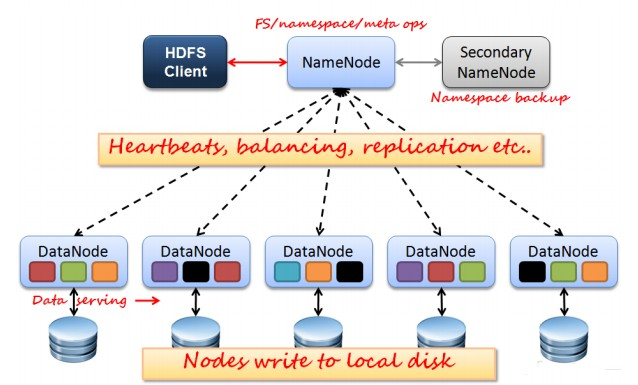
\includegraphics[height=7cm,width= 10cm]{img/hdfs.jpg}
    \caption{spark1}
\label{spark1}
\end{figure}
    HDFS也是按照Master和Slave的结构。分NameNode、SecondaryNameNode、DataNode这几个角色。
    NameNode:是Master节点,管理数据块映射;处理客户端的读写请求;配置副本策略;管理HDFS的名称空间;

SecondaryNameNode:分担namenode的工作量;是NameNode的冷备份;合并fsimage和fsedits然后再发给Namenode。

DataNode:Slave节点,负责存储client发来的数据块block;执行数据块的读写操作。

热备份:b是a的热备份,如果a坏掉。那么b马上运行代替a的工作。

冷备份:b是a的冷备份,如果a坏掉。那么b不能马上代替a工作。但是b上存储a的一些信息,减少a坏掉之后的损失。

fsimage:元数据镜像文件(文件系统的目录树。)

edits:元数据的操作日志(针对文件系统做的修改操作记录)

namenode内存中存储的是=fsimage+edits。

SecondaryNameNode负责定时默认1小时,从namenode上,获取fsimage和edits来进行合并,然后再发送给namenode。减少namenode的工作量。

原理
 若client为DataNode节点,那存储block时,规则为:副本1,同client的节点上;副本2,不同机架节点上;副本3,同第二个副本机架的另一个节点上;其他副本随机挑选。

若client不为DataNode节点,那存储block时,规则为:副本1,随机选择一个节点上;副本2,不同副本1,机架上;副本



\subsection{GFS与HDFS的区别}
HDFS 参照了它所以大部分架构设计概念是类似的,
比如 HDFS NameNode 相当于 GFS Master,HDFS DataNode 相当于 GFS chunkserver。

1.写入模型

HDFS 在考虑写入模型时做了一个简化,就是同一时刻只允许一个写入者或追加者。 
在这个模型下同一个文件同一个时刻只允许一个客户端写入或追加。
而 GFS 则允许同一时刻多个客户端并发写入或追加同一文件。

2.GFS的写入流程

允许并发写入带来了更复杂的一致性问题。 
所谓一致性就是,对同一个文件,所有的客户端看到的数据是一致的,不管它们是从哪个副本读取的。

3.写入流程

GFS 和 HDFS 的写入流程都采用了流水线方式,但 HDFS 没有分离数据流和控制流。
HDFS 的数据流水线写入在网络上的传输顺序与最终写入文件的顺序一致。
而 GFS 数据在网络上的传输顺序与最终写入文件的顺序可能不一致。
GFS 在支持并发写入和优化网络数据传输方面做出了最佳的折衷。

总结:

GFS 的论文发表于 2003 年,后来大部分的分布式文件系统设计实现或多或少都参考了 GFS 的设计思路。
而 HDFS 算是开源分布式文件系统中最完整实现了 GFS 论文中的概念模型。 
但 HDFS 依然简化了 GFS 中关于并发写的思路

\subsection{Hadoop中MapReduce编程模型}
MapReduce编程模型对外提供两层,底层为基本的java API,有5个可编程组件:InputFormat, Mapper, Partitioner, Reducer, OutputFormat
上层为4个工具包。

序列化:是指将结构化对象转换为字节流以便于通过网络进行传输或写入持久存储的过程。Hadoop MapReduce中,序列化的主要作用有两个:永久存储和进程间通信。
回调机制,用于回调用户提供的map或reduce函数。

MapReduce作业配置与提交,作业由两部分组成:应用程序和作业配置。作业配置:环境配置和用户自定义配置。用户自定义配置包括:作业名称,mapper/reducer, reduce task个数。
